\label{ch:glide}

This chapter describes the numerical implementation of mass, momentum, and energy conservation in the Glide dynamical core. For a model governed by shallow-ice dynamics, the solutions for the conservation of mass and momentum are intimately linked.

\section{Ice Thickness Evolution}
\label{sc:glide_thickness_evolution}
The evolution of the ice thickness, $H$, stems from the continuity equation and can be expressed as
\begin{equation}
  \label{kin.eq.ice_thickness}
  \frac{\pd H}{\pd t} = -\vec\nabla\cdot(\overline{\vec{u}} H) + B,
\end{equation}
where $\overline{\vec{u}}$ is the vertically averaged ice velocity, $B$ is the surface mass balance and $\vec\nabla$ is the horizontal gradient operator \citep{Payne1997}. 

%For large--scale ice sheet models, the \emph{shallow ice approximation} is generally used. 
For some regions of large--scale ice sheets, such as the slow moving interior, or for simulations run at coarse spatial resolution, a model governed by the \emph{shallow ice approximation} may be appropriate. Further, for very-long time integrations, such as those required in paleoclimate studies, a model governed by the shallow ice approximation may
be the only computationally practical approach.
%The shallow ice approximation assumes that bedrock and ice surface slopes are sufficiently small so that the normal stress components can be neglected \citep{Hutter1983}. 

Based largely on the assumption that bedrock and ice surface slopes are sufficiently small \citep{Hutter1983}, the shallow ice approximation neglects all stress components other than those associated with vertical shearing in the horizontal directions. 
These stresses, $\tau_{xz}$ and $\tau_{yz}$, are approximated by
\begin{equation}
  \label{kin.eq.horiz_shear}
  \begin{split}
    \tau_{xz}(z)&=-\rho g(s-z)\frac{\pd s}{\pd x},\\
    \tau_{yz}(z)&=-\rho g(s-z)\frac{\pd s}{\pd y},
  \end{split}
\end{equation}
where $\rho$ is the density of ice, $g$ the acceleration due to gravity and $s=H+h$ the ice surface. \textbf{Steve: I think the latter should be H + b? Unless they use h in this chapter to denote the bedrock elevation. If that is the case, we should probably update so that it is consistent w/ the rest of the documentation, which uses b for bedrock elev.}

Strain rates $\dot{\epsilon}_{ij}$ of polycrystalline ice are related to the stress tensor by the non--linear flow law:
\begin{equation}
  \label{kin.eq.flowlaw}
  \dot{\epsilon}_{iz}=\frac12\left(\frac{\pd u_i}{\pd z}+\frac{\pd u_z}{\pd i}\right)=A(T^\ast)\tau_\ast^{(n-1)}\tau_{iz}\qquad i=x,y,
\end{equation}
where $\tau_\ast$ is the effective shear stress defined by the second invariant of the stress tensor, $n$ the flow law exponent and $A$ the temperature--dependent flow law coefficient. $T^\ast$ is the absolute temperature corrected for the dependence of the melting point on pressure \cite[$T^\ast=T+8.7\cdot10^{-4}(H+h-z)$, $T$ in Kelvin,][]{Huybrechts1986}. 
%The parameters $A$ and $n$ have to be found by experiment. 
The parameters $n$ and $A$ are determined experimentally; $n$ is usually taken to be 3 and $A$ depends primarily on temperature and secondarily on factors such as crystal
size and orientation and ice impurities. 
%on factors such as temperature, crystal size and orientation, and ice impurities. 
Experiments suggest that $A$ follows the Arrhenius relationship:
\begin{equation}
  \label{kin.eq.arrhenius}
  A(T^\ast)=fae^{-Q/RT^\ast},
\end{equation}where $a$ is a temperature--independent material constant, $Q$ is the activation energy for creep and $R$ is the universal gas constant \citep{Paterson1994}. 
$f$ is a tuning parameter that may be used to ``speed--up" ice flow, accounting for the effects of ice impurities and the development of anisotropic ice fabrics \citep{Payne1999,Tarasov1999,Tarasov2000,Peltier2000}.

Integrating \eqref{kin.eq.arrhenius} with respect to $z$ gives the vertical profile of the horizontal velocity in each column:
\begin{equation}
  \label{kin.eq.horiz_velo}
  \vec u(z)-\vec u(h) = -2(\rho g)^n|\vec\nabla s|^{n-1}\vec\nabla s\int_h^zA(s-z)^ndz,
\end{equation}
where $\vec u(h)$ is the basal velocity (sliding velocity). Integrating \eqref{kin.eq.horiz_velo} again with respect to $z$ gives an expression for the vertically averaged ice velocity:
\begin{equation}
  \label{kin.eq.avg_velo}
  \overline{\vec u}H=-2(\rho g)^n|\vec\nabla s|^{n-1}\vec\nabla s\int_h^s\int_h^zA(s-z)^ndzdz'.
\end{equation}

The vertical ice velocity can be derived from the conservation of mass for an incompressible material:
\begin{equation}
  \label{kin.eq.incompress}
  \frac{\pd u_x}{\pd x} + \frac{\pd u_y}{\pd y} + \frac{\pd u_z}{\pd z} = 0.
\end{equation}
Integrating \eqref{kin.eq.incompress} with respect to $z$ gives the vertical profile of the vertical velocity in each column:
\begin{equation}
  \label{kin.eq.vert_velo}
  w(z)=-\int_h^z\vec\nabla\cdot\vec u(z)dz+w(h),
\end{equation}
with lower, kinematic boundary condition
\begin{equation}
  w(h)=\frac{\pd h}{\pd t}+\vec u(h)\cdot\vec\nabla h+S,
\end{equation}
where $S$ is the melt rate at the ice base given by Equation \eqref{temp.eq.meltrate}. The upper kinematic boundary is given by the surface mass balance and must satisfy:
\begin{equation}
  \label{kin.eq.upper_bc}
  w(s)=\frac{\pd s}{\pd t}+\vec u(s)\cdot\vec\nabla s+B.
\end{equation}
\textbf{Steve: need to replace the h with b in the above expressions and also make sure other notation is consistent w/ the rest of the documentation.}

\subsection{Numerical Grid}\label{num.sec.grid}
The continuous equations describing ice physics have to be discretized in order to be solved by a computer (which is inherently finite). This section describes the finite--difference grids used by the model.
\subsubsection{Horizontal Grid}
The modelled region ($x\in[0,L_x]$, $y\in[0,L_y]$) is discretized using a regular grid so that $x_i=(i-1)\Delta x$ for $i\in[1,N]$ (and similarly for $y_j$). The model uses two staggered horizontal grids in order to improve stability. Both grids use the same grid spacing, $\Delta x$ and $\Delta y$, but are offset by half a grid cell (see Fig. \ref{kin.fig.grid}). 
\begin{figure}[htbp]
  \begin{center}
    
\includegraphics{\dir/figs/grid.eps}
    \caption{Horizontal Grid.}
    \label{kin.fig.grid}
  \end{center}
\end{figure}
Quantities calculated on the staggered $(r,s)$--grid are denoted with a tilde, i.e., $\tilde{F}$. Quantities are transformed between grids by averaging over the surrounding nodes; i.e., a quantity in the $(i,j)$--grid becomes in the $(r,s)$--grid:
\begin{subequations}
  \begin{align}
    \tilde{F}_{r,s}&=\tilde{F}_{i+\frac12,j+\frac12}=\frac14(F_{i,j}+F_{i+1,j}+F_{i+1,j+1}+F_{i,j+1}),\\
    \intertext{and similarly for the reverse transformation:}
    F_{i,j}&=F_{r-\frac12,s-\frac12}=\frac14(\tilde{F}_{r-1,s-1}+\tilde{F}_{r,s-1}+\tilde{F}_{r,s}+\tilde{F}_{r-1,s}).
  \end{align}
\end{subequations}

In general, horizontal velocities and associated quantities like the diffusivity are calculated on the $(r,s)$--grid. Ice thickness, temperatures and vertical velocities are calculated on the $(i,j)$--grid.

Horizontal gradients are calculated on the $(r,s)$--grid; i.e., surface gradients are
\begin{subequations}
\begin{align}
  \left(\frac{\pd s}{\pd x}\right)_{r,s}=\tilde{s}^x_{r,s}&=\frac{s_{i+1,j}-s_{i,j}+s_{i+1,j+1}-s_{i,j+1}}{2\Delta x},\\
  \left(\frac{\pd s}{\pd y}\right)_{r,s}=\tilde{s}^y_{r,s}&=\frac{s_{i,j+1}-s_{i,j}+s_{i+1,j+1}-s_{i+1,j}}{2\Delta y}.
\end{align}  
\end{subequations}
Ice thickness gradients, $\tilde{H}^x_{r,s}$ and $\tilde{H}^y_{r,s}$, are formed analogously. Gradients in the $(r,s)$--grid are formed in a similar way: 
\begin{equation}
  \left(\frac{\pd u}{\pd x}\right)_{i,j}=u^x_{i,j}=\frac{\tilde{u}_{r,s-1}-\tilde{u}_{r-1,s-1}+\tilde{u}_{r,s}-\tilde{u}_{r-1,s}}{2\Delta x}.
\end{equation}

\subsubsection{Periodic Boundary Conditions}
The model can be run with horizontal periodic boundary conditions, i.e. with the western edge of the modelled region joined to the eastern edge. Figure \ref{num.fig.grid_ew} illustrates the numeric grid when the model is run in torus mode.

\begin{figure}[htbp]
  \centering
  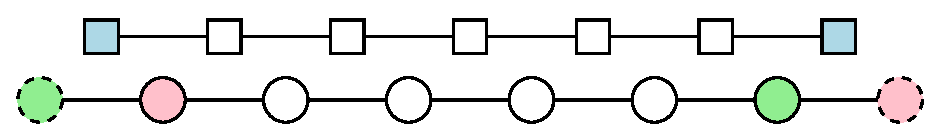
\includegraphics[width=0.9\textwidth]{\dir/figs/grid_ew.eps}
  \caption{A row of the numeric grid when the model is used in torus mode. Circles indicate points in $(i,j)$--grid and squares indicate points in the $(r,s)$--grid. Points with the same color are logically the same.}
  \label{num.fig.grid_ew}
\end{figure}

These boundary conditions are enforced by exchanging points for the temperature and vertical velocity calculations. The ice thicknesses are calculated explicitly at the ghostpoints.

\subsubsection{$\sigma$--Coordinate System}\label{num.sec.sigma}
The vertical coordinate, $z$, is scaled by the ice thickness analogous to the $s$--coordinate in numerical weather simulations \citep[e.g.,][]{Holton1992}. A new vertical coordinate, $\sigma$, is introduced so that the ice surface is at $\sigma=0$ and the ice base at $\sigma=1$ (see Fig. \ref{kin.fig.scale}), i.e.
\begin{equation}
  \label{kin.eq.vertical_scale}
  \sigma=\frac{s-z}{H}.
\end{equation}

\begin{figure}[htbp]
  \begin{center}
    
\includegraphics{\dir/figs/scale.eps}
    \caption[Vertical scaling of the ice sheet model.]{Vertical scaling of the ice sheet model. The vertical axis is scaled to unity. The horizontal coordinates are not changed.}
    \label{kin.fig.scale}
  \end{center}
\end{figure}


The derivatives of a function $f$ in $(x,y,z,t)$ become in the new $(\tilde{x},\tilde{y},\sigma,\tilde{t})$ system:
\begin{subequations}
  \begin{align}
    \frac{\pd f}{\pd x} &= \frac{\pd f}{\pd\tilde{x}}+\frac1H\Delta_{\tilde{x}}\frac{\pd f}{\pd \sigma},\\
    \frac{\pd f}{\pd y} &= \frac{\pd f}{\pd\tilde{y}}+\frac1H\Delta_{\tilde{y}}\frac{\pd f}{\pd \sigma},\\
    \frac{\pd f}{\pd t} &= \frac{\pd f}{\pd\tilde{t}}+\frac1H\Delta_{\tilde{t}}\frac{\pd f}{\pd \sigma},\\
    \frac{\pd f}{\pd z} &= -\frac1H\frac{\pd f}{\pd\sigma},
  \end{align}
\end{subequations}
where  the geometric factors, $\Delta_{\tilde{x}}$, $\Delta_{\tilde{y}}$ and $\Delta_{\tilde{t}}$, are defined by
\begin{subequations}
  \begin{align}
  \Delta_{\tilde{x}}&=\left(\frac{\pd s}{\pd\tilde{x}}-\sigma\frac{\pd H}{\pd\tilde{x}}\right),\\
  \Delta_{\tilde{y}}&=\left(\frac{\pd s}{\pd\tilde{y}}-\sigma\frac{\pd H}{\pd\tilde{y}}\right),\\
  \Delta_{\tilde{t}}&=\left(\frac{\pd s}{\pd\tilde{t}}-\sigma\frac{\pd H}{\pd\tilde{t}}\right).
  \end{align}
\end{subequations}
The integral of $z$ becomes in the $\sigma$--coordinate system:
\begin{equation}
  \int_b^zfdz=-H\int_1^\sigma fd\sigma.
\end{equation}

The vertical coordinate can be discretized using an irregular grid spacing to reflect the fact that ice flow is more variable at the bottom of the ice column. In the vertical the index $k$ is used. 


\subsection{Ice Sheet Equations in $\sigma$--Coordinates}
The horizontal velocity, Equation \eqref{kin.eq.horiz_velo}, becomes in the $\sigma$--coordinate system
\begin{equation}
  \label{kin.eq.vert_velo_sigma}
  \vec u(\sigma) = -2(\rho g)^nH^{n+1}|\vec\nabla s|^{n-1}\vec\nabla s\int_1^\sigma A\sigma^nd\sigma+\vec u(1)
\end{equation}
and the vertically averaged velocity
\begin{equation}
  \label{kin.eq.avg_velo_scaled}
  \overline{\vec u} H=H\int_0^1\vec ud\sigma+\vec u(1)H
\end{equation}
The vertical velocity, Equation \eqref{kin.eq.vert_velo}, becomes
\begin{equation}
  \label{kin.eq.vert_velo_scaled}
  w(\sigma)=-\int_1^\sigma\left(\frac{\pd\vec u}{\pd\sigma}\cdot(\vec\nabla s-\sigma\vec\nabla H)+H\vec\nabla\cdot\vec u\right)d\sigma+w(1)
\end{equation}
and lower boundary condition
\begin{equation}
  w(1)=\frac{\pd h}{\pd t}+\vec u(1)\cdot\vec\nabla h+S.
\end{equation}

\subsection{Calculating the Horizontal Velocity and the Diffusivity}
Horizontal velocity and diffusivity calculations are split up into two parts:
\begin{subequations}
  \label{kin.eq.horiz_diffusivity}
  \begin{align}
    \vec u(\sigma)&=c\vec\nabla s+\vec u(1)\\
    D &=H\int_0^1cd\sigma\\
    \vec q&=D\vec\nabla s+H\vec u(1)\\
    \intertext{with}
    c(\sigma)&=-2(\rho g)^nH^{n+1}|\vec\nabla s|^{n-1}\int_1^\sigma A\sigma^nd\sigma
  \end{align}
\end{subequations}

Quantities $\vec u$ and $D$ are found on the velocity grid. Integrating from the ice base ($k=N-1$), the discretised quantities become
\begin{subequations}
  \begin{equation}
    \tilde{c}_{r,s,N}=0
  \end{equation}
  \begin{multline}
    \tilde{c}_{r,s,k}=-2(\rho g)^nH_{r,s}^{n+1}\left(({\tilde{s}^x_{r,s}})^2+({\tilde{s}^y_{r,s}})^2\right)^{\frac{n-1}{2}}\\
    \sum_{\kappa=N-1}^k\frac{A_{r,s,\kappa}+A_{r,s,\kappa+1}}2 \left(\frac{\sigma_{\kappa+1}+\sigma_\kappa}2\right)^n(\sigma_{\kappa+1}-\sigma_\kappa)
  \end{multline}
  \begin{equation}
    \tilde{D}_{r,s}=H_{r,s}\sum_{k=0}^{N-1}\frac{\tilde{c}_{r,s,k}+\tilde{c}_{r,s,k+1}}2(\sigma_{k+1}-\sigma_k)
  \end{equation}
\end{subequations}
Expressions for $\vec{u}_{i,j,k}$ and $\vec{q}_{i,j}$ are straight forward.

\subsection{Solving the Ice Thickness Evolution Equation}
Equation \eqref{kin.eq.ice_thickness} can be rewritten as a diffusion equation, with non--linear diffusion coefficient $D$:
\begin{equation}
  \label{kin.eq.ice_evo}
  \frac{\pd H}{\pd t}=-\vec\nabla\cdot D\vec\nabla s+B=-\vec\nabla\cdot\vec q+B
\end{equation}
This non--linear partial differential equation can be linearised by using the diffusion coefficient from the previous time step. The diffusion coefficient is calculated on the $(r,s)$--grid, i.e. staggered in both $x$ and $y$ direction. Figure \ref{kin.fig.staggered_grid} illustrates the staggered grid. Using finite differences, the fluxes in $x$ direction, $q^x$ become
\begin{subequations}
\begin{align}
  q^x_{i+\frac12,j}&=-\frac12(\tilde{D}_{r,s}+\tilde{D}_{r,s-1})\frac{s_{i+1,j}-s_{i,j}}{\Delta x}\\
  q^x_{i-\frac12,j}&=-\frac12(\tilde{D}_{r-1,s}+\tilde{D}_{r-1,s-1})\frac{s_{i,j}-s_{i-1,j}}{\Delta x}\\
  \intertext{and the fluxes in $y$ direction}
  q^y_{i,j+\frac12}&=-\frac12(\tilde{D}_{r,s}+\tilde{D}_{r-1,s})\frac{s_{i,j+1}-s_{i,j}}{\Delta y}\\
  q^y_{i,j-\frac12}&=-\frac12(\tilde{D}_{r,s-1}+\tilde{D}_{r-1,s-1})\frac{s_{i,j}-s_{i,j-1}}{\Delta y}.
\end{align}  
\end{subequations}

\begin{figure}[htbp]
  \centering
  
\includegraphics{\dir/figs/staggered_grid.eps}
  \caption{Illustration of the staggered grid used to calculate ice thicknesses, diffusivities and mass fluxes.}
  \label{kin.fig.staggered_grid}
\end{figure}

\subsubsection{ADI Scheme}
The alternating--direction implicit method (ADI) uses the concept of operator splitting where Equation \eqref{kin.eq.ice_evo} is first solved in the $x$--direction and then in the $y$--direction, \citep{Press1992}. The time step $\Delta t$ is devided into two time steps $\Delta t/2$. The descretised version of Equation \eqref{kin.eq.ice_evo} becomes \citep{Huybrechts1986}:
\begin{subequations}
\begin{align}
  \label{kin.eq.adi_1}
  2\frac{H_{i,j}^{t+\frac12}-H_{i,j}^{t}}{\Delta t} &= -\frac{q_{i+\frac12,j}^{x,t+\frac12}-q_{i-\frac12,j}^{x,t+\frac12}}{\Delta x} - \frac{q_{i,j+\frac12}^{y,t}-q_{i,j-\frac12}^{y,t}}{\Delta y} + B_{i,j} \\
  \label{kin.eq.adi_2}
  2\frac{H_{i,j}^{t+1}-H_{i,j}^{t+\frac12}}{\Delta t} &= -\frac{q_{i+\frac12,j}^{x,t+\frac12}-q_{i-\frac12,j}^{x,t+\frac12}}{\Delta x} - \frac{q_{i,j+\frac12}^{y,t+1}-q_{i,j-\frac12}^{y,t+1}}{\Delta y} + B_{i,j}
\end{align}
\end{subequations}
Gathering all $t+\frac12$ terms on the left side, Equation \eqref{kin.eq.adi_1} can be expressed as a tri--diagonal set of equations for each row $j$:
\begin{equation}
  -\alpha_{i,j}H_{i-1,j}^{t+\frac12} + (1-\beta_{i,j})H_{i,j}^{t+\frac12} - \gamma_{i,j}H_{i+1,j}^{t+\frac12} = \delta_{i,j}
\end{equation}
with
\begin{subequations}
  \begin{align}
  \alpha_{i,j} &=\frac{\tilde{D}_{r-1,s}+\tilde{D}_{r-1,s-1}}{4\Delta x^2}\Delta t\\
  \beta_{i,j}  &=-\frac{\tilde{D}_{r,s}+2\tilde{D}_{r-1,s}+\tilde{D}_{r-1,s-1}}{4\Delta x^2}\Delta t = -(\alpha_{i,j}+\gamma_{i,j})\\
  \gamma_{i,j} &=\frac{\tilde{D}_{r,s}+\tilde{D}_{r,s-1}}{4\Delta x^2}\Delta t    
  \end{align}
and the RHS,
\begin{equation}
  \delta_{i,j} = H_{i,j}^t-\frac{\Delta t}{2\Delta y}\left(q_{i,j+\frac12}^{y,t}-q_{i,j-\frac12}^{y,t}\right) + \frac{\Delta t}2B_{i,j} + \alpha_{i,j}h_{i-1,j} -\beta_{i,j}h_{i,j} + \gamma_{i,j}h_{i+1,j}.
\end{equation}
\end{subequations}

A similar tri--diagonal system is found for each column, $i$ of Equation \eqref{kin.eq.adi_2}.

\subsubsection{Linearised Semi--Implicit Scheme}
Using the Crank--Nicolson scheme, the semi--implicit temporal discretisation of \eqref{kin.eq.ice_evo} is then:
\begin{multline}
\label{kin.eq.ice_evo_disc1}
  \frac{H^{t+1}_{i,j}-H^t_{i,j}}{\Delta t}=\frac{q^{x,t+1}_{i+\frac12,j}-q^{x,t+1}_{i-\frac12,j}}{2\Delta x}+\frac{q^{y,t+1}_{i,j+\frac12}-q^{y,t+1}_{i,j-\frac12}}{2\Delta y} \\
  +\frac{q^{x,t}_{i+\frac12,j}-q^{x,t}_{i-\frac12,j}}{2\Delta x}+\frac{q^{y,t}_{i,j+\frac12}-q^{y,t}_{i,j-\frac12}}{2\Delta y}+ B_{i,j}
\end{multline}
The superscripts $^t$ and $^{t+1}$ indicate at what time the ice thickness $H$ is evaluated. Collecting all $H^{t+1}$ terms of \eqref{kin.eq.ice_evo_disc1} on the LHS and moving all other terms to the RHS we can rewrite \eqref{kin.eq.ice_evo_disc1} as
\begin{equation}
  \label{kin.eq.evo_matrix}
  -\alpha_{i,j}H^{t+1}_{i-1,j} - \beta_{i,j}H^{t+1}_{i+1,j} - \gamma_{i,j}H^{t+1}_{i,j-1} - \delta_{i,j}H^{t+1}_{i,j+1}+ (1-\epsilon_{i,j})H^{t+1}_{i,j} = \zeta_{i,j}
\end{equation}
with the RHS,
\begin{multline}
  \zeta_{i,j} = \alpha_{i,j}H^{t}_{i-1,j} + \beta_{i,j}H^{t}_{i+1,j} + \gamma_{i,j}H^{t}_{i,j-1} + \delta_{i,j}H^{t}_{i,j+1} + (1+\epsilon_{i,j})H^{t}_{i,j} \\
  + 2(\alpha_{i,j}h_{i-1,j} + \beta_{i,j}h_{i+1,j} + \gamma_{i,j}h_{i,j-1} + \delta_{i,j}h_{i,j+1}+ \epsilon_{i,j}h_{i,j}) + B_{i,j}\Delta t
\end{multline}
with the elements of the sparse matrix
\begin{subequations}
  \begin{align}
    \alpha_{i,j} &=\frac{\tilde{D}_{r-1,s}+\tilde{D}_{r-1,s-1}}{4\Delta x^2}\Delta t\\
    \beta_{i,j} &=\frac{\tilde{D}_{r,s}+\tilde{D}_{r,s-1}}{4\Delta x^2}\Delta t\\
    \gamma_{i,j} &=\frac{\tilde{D}_{r,s-1}+\tilde{D}_{r-1,s-1}}{4\Delta y^2}\Delta t\\
    \delta_{i,j} &=\frac{\tilde{D}_{r,s}+\tilde{D}_{r-1,s}}{4\Delta y^2}\Delta t\\
    \epsilon_{i,j} &=-(\alpha_{i,j}+\beta_{i,j}+\gamma_{i,j}+\delta_{i,j})
  \end{align}
\end{subequations}

This matrix equation is solved using an iterative matrix solver for non-symmetric sparse matrices. The solver used here is the bi--conjugate gradient method with incomplete LU decomposition preconditioning provided by the SLAP package.

\subsubsection{Non--Linear Scheme}
The non--linearity of Equation \eqref{kin.eq.ice_evo} arises from the dependance of $D$ on $s$. A non--linear scheme for \eqref{kin.eq.ice_evo} can be formulated using Picard iteration, which consists of two iterations: an outer, non--linear and an inner, linear equation. The scheme is started off with the diffusivity from the previous time step, i.e.
\begin{subequations}
  \begin{equation}
    D^{(0),t+1}=D^{t}
  \end{equation}
and Equation \eqref{kin.eq.evo_matrix} becomes
\begin{multline}
  \label{kin.eq.evo_matrix_nonlin}
  -\alpha^{(\xi),t+1}_{i,j}H^{t+1}_{i-1,j} - \beta^{(\xi),t+1}_{i,j}H^{(\xi+1),t+1}_{i+1,j} - \gamma^{(\xi),t+1}_{i,j}H^{(\xi+1),t+1}_{i,j-1} \\
  - \delta^{(\xi),t+1}_{i,j}H^{(\xi+1),t+1}_{i,j+1}+ (1-\epsilon^{(\xi),t+1}_{i,j})H^{(\xi+1),t+1}_{i,j} = \zeta^{(0),t}_{i,j}
\end{multline}
\end{subequations}
Equation \eqref{kin.eq.evo_matrix_nonlin} is iterated over $\xi$ until the maximum ice thickness residual is smaller than some threshold:
\begin{equation}
  \max\left(\left|H^{(\xi+1),t+1}-H^{(\xi),t+1}\right|\right)<H_{\text{res}}
\end{equation}

\begin{figure}[htbp]
  \centering
  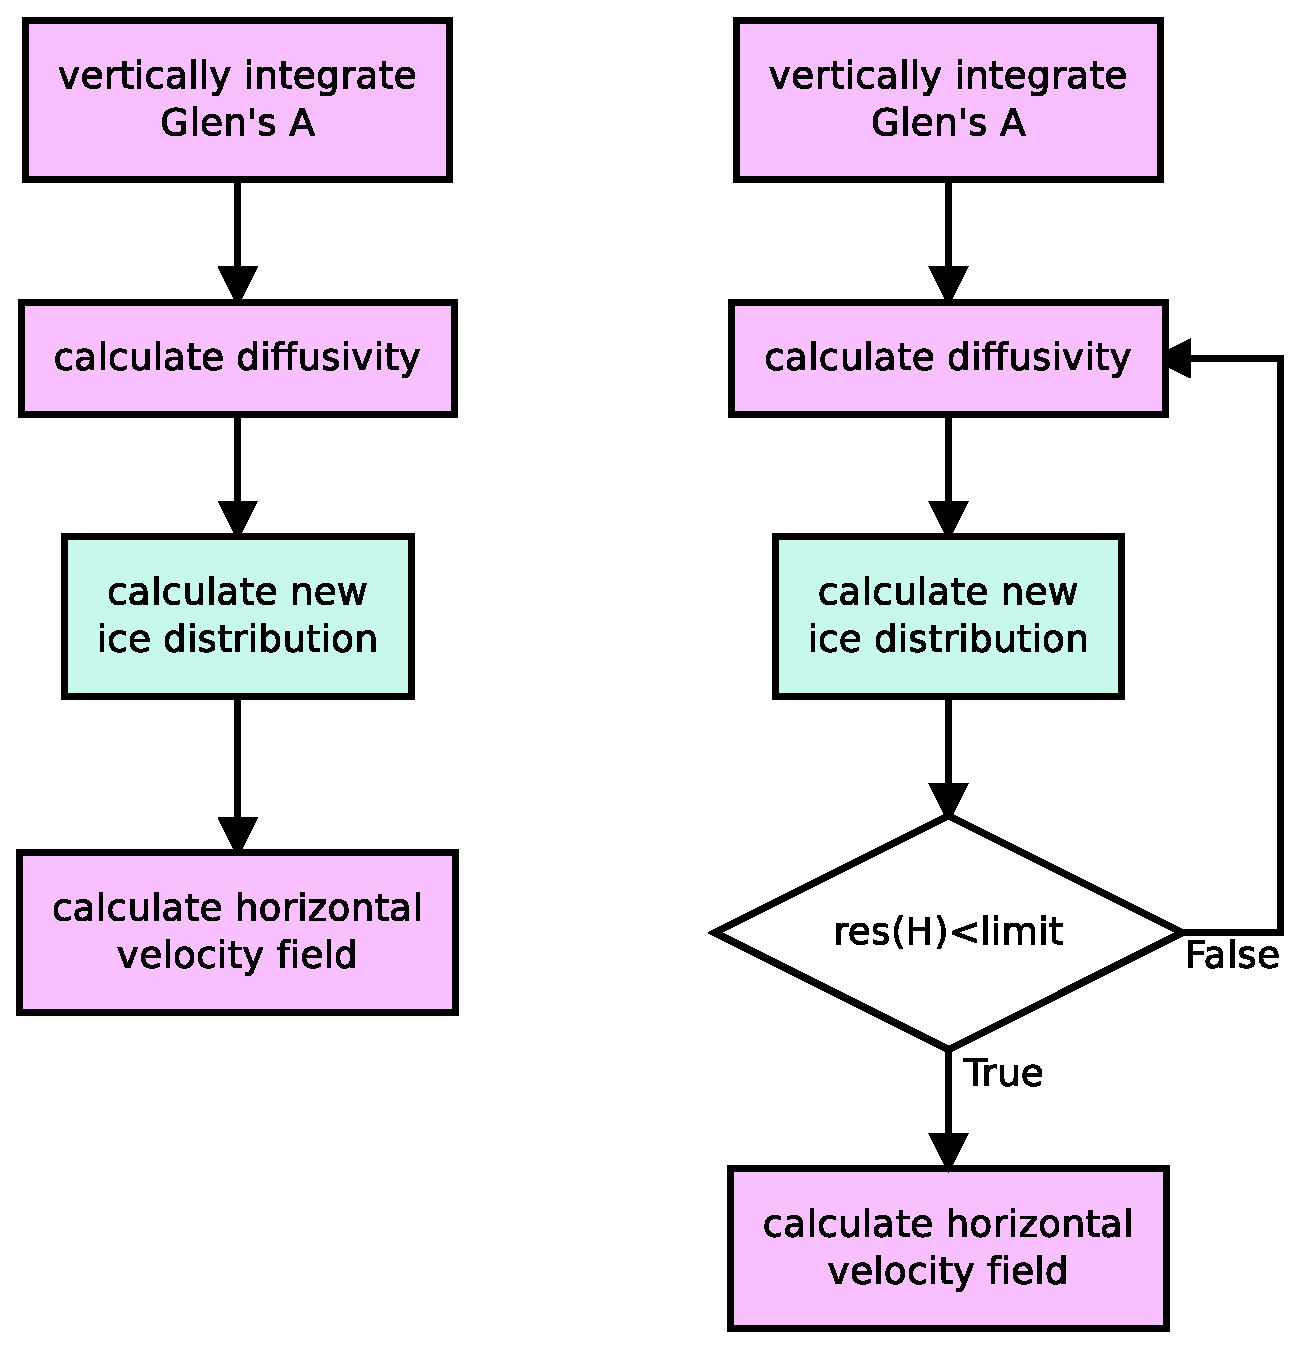
\includegraphics[width=0.5\textwidth]{\dir/figs/thick_evo.eps}
  \caption{Flow diagram showing how the linearised solver (on the left) and the non--linear solver work. The inner, linear iteration is contained within the box labeled ``calculate new ice distribution''.}
  \label{kin.fig.solvers}
\end{figure}

\subsection{Calculating Vertical Velocities}

\subsubsection{Grid Velocity}
The vertical grid moves as a result of using a $\sigma$--coordinate system. The grid velocity is
\begin{equation}
  \label{kin.eq.grid_velo}
  w^{\text{grid}}(\sigma)=\frac{\pd s}{\pd t}+\vec u\cdot\vec\nabla s-\sigma\left(\frac{\pd H}{\pd t}+\vec u\cdot\vec\nabla H\right).
\end{equation}
The numerical implementation of \eqref{kin.eq.grid_velo} is straightforward.

\subsubsection{Vertical Velocity}
The discretized version of the vertical velocity equation \eqref{kin.eq.vert_velo_scaled} is slightly more compilicated because the horizontal velocities are calculated on the $(r,s)$ grid. The vertical velocity at the ice base is $w_{i,j,N}=w^{\text{grid}}_{i,j,N}-M_b{i,j}$, where $M_b{i,j}$ is the basal melt rate. Integrating from the bottom, the vertical velocity is then
\begin{equation}
  \label{kin.eq.wvel_unc}
  \begin{split}
  w_{i,j,k}=-\sum_{\tilde{k}=N-1}^1\left\{\mathcal{H}_{i,j}\left(\frac{u^x_{i,j,k}+u^x_{i,j,k+1}}{2}+\frac{v^y_{i,j,k}+v^y_{i,j,k+1}}{2}\right)(\sigma_{k+1}-\sigma_k)\right. \\
     +(\tilde{u}_{i,j,k+1}-\tilde{u}_{i,j,k})  \left(\tilde{s}^x_{i,j}-\frac12(\sigma_{k+1}+\sigma_k)\tilde{H}^x_{i,j}\right)  \\
     \left.+(\tilde{v}_{i,j,k+1}-\tilde{v}_{i,j,k})  \left(\tilde{s}^y_{i,j}-\frac12(\sigma_{k+1}+\sigma_k)\tilde{H}^y_{i,j}\right)\right\} + w_{i,j,N},
  \end{split}
\end{equation}
with the weighted ice thickness
\begin{equation*}
  \begin{split}
  \mathcal{H}_{i,j}=\frac{4H_{i,j}+2(H_{i-1,j}+H_{i+1,j}+H_{i,j-1}+H_{i,j+1})}{16}\\
  +\frac{H_{i-1,j-1}+H_{i+1,j-1}+H_{i+1,j+1}+H_{i-1,j+1}}{16}.    
  \end{split}
\end{equation*}

This scheme produces vertical velocities at the ice divide which are too small. The vertical velocities on the ice surface are given by the upper kinematic boundary condition \eqref{kin.eq.upper_bc}. Equation \eqref{kin.eq.wvel_unc} can be corrected with
\begin{equation}
  \label{kin.eq.wvel_cor}
   w^\ast_{i,j,k}=w_{i,j,k}-(1-\sigma_k)(w_{i,j,k}-{w_s}_{i,j}),
\end{equation}
where ${w_s}_{i,j}$ is the vertical velocity at the ice surface given by \eqref{kin.eq.upper_bc}. Figure \ref{kin.fig.w_profile} shows the different vertical velocities at the ice surface.
\begin{figure}[htbp]
  \centering
  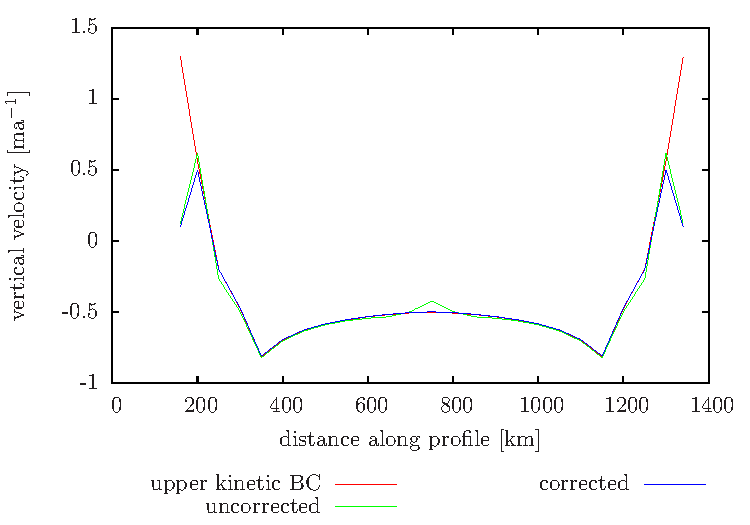
\includegraphics{\dir/gnu/w_profile.eps}
  \caption{Vertical ice surface velocities of the EISMINT-1 moving margin experiment.}
  \label{kin.fig.w_profile}
\end{figure}
The difference between the vertical velocities calculated by the model and the vertical velocities given by \eqref{kin.eq.upper_bc} at the ice margin are due to the fact that temperatures and velocities are only calculated when the ice is thicker than a certain threshold value which is not met at the ice margin.

Figure \ref{kin.fig.wt_sigma} shows vertical profiles of the vertical velocity at the ice divide and a point halfway between the divide and the domain margin. A corresponding temperature profile is also shown since the vertical velocity determines the vertical temperature advection (see Section \ref{temp.sec.vert_ad}).
\begin{figure}[htbp]
  \centering
  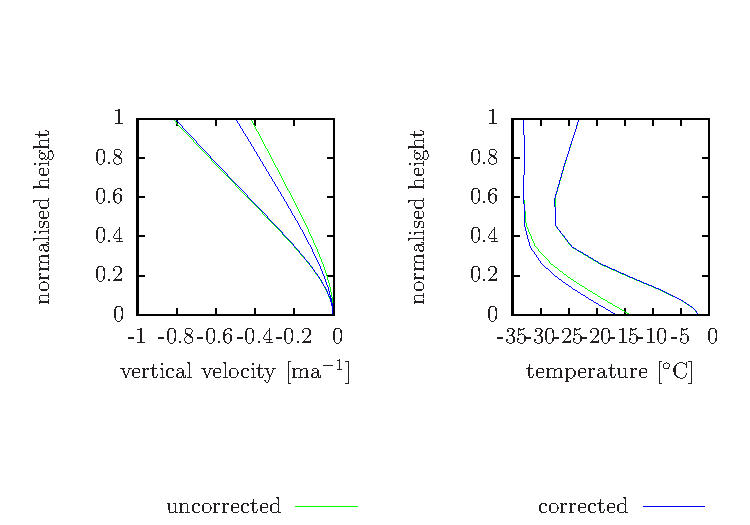
\includegraphics{\dir/gnu/wt_sigma.eps}
  \caption{Vertical velocity and temperature distribution for columns at the ice divide and a point halfway between the divide and the domain margin.}
  \label{kin.fig.wt_sigma}
\end{figure}


\section{Temperature Solver}
The flow law, Equation \eqref{kin.eq.flowlaw}, depends on the temperature of ice. It is, therefore, necessary to determine how the distribution of ice temperatures changes with a changing ice sheet configuration. The thermal evolution of the ice sheet is described by
\begin{equation}
  \label{temp.eq.temp_z}
  \frac{\pd T}{\pd t}=\frac{k}{\rho c}\nabla^2T-\vec{u}\cdot\vec\nabla T+\frac\Phi{\rho c}-w\frac{\pd T}{\pd z},
\end{equation}
where $T$ is the absolute temperature, $k$ is the thermal conductivity of ice, $c$ is the specific heat capacity and $\Phi$ is the heat generated due to internal friction. In the $\sigma$--coordinate system, Equation \eqref{temp.eq.temp_z}, becomes
\begin{equation}
  \label{temp.eq.temp}
  \frac{\pd T}{\pd t} = \frac{k}{\rho cH^2}\frac{\pd^2T}{\pd\sigma^2} - \vec{u}\cdot\vec\nabla T + \frac{\sigma g}c\frac{\pd \vec{u}}{\pd\sigma}\cdot\vec\nabla s + \frac1H\frac{\pd T}{\pd\sigma}\left(w-w_{\text{grid}}\right)
\end{equation}
The terms represents (1) vertical diffusion, (2) horizontal advection, (3) internal heat generation due to friction and (4) vertical advection and a correction due to the sigma coordinate system. Let's rewrite \eqref{temp.eq.temp} to introduce some names:
\begin{equation}
  \label{temp.eq.temp2}
  \frac{\pd T}{\pd t} = a\frac{\pd^2T}{\pd\sigma^2} +b(\sigma) + \Phi(\sigma) + c(\sigma)\frac{\pd T}{\pd\sigma},
\end{equation}
where
\begin{subequations}
  \begin{align}
    a&=\frac{k}{\rho cH^2} \\
    \label{temp.eq.hadv}
    b(\sigma)&=-\vec{u}\cdot\vec\nabla T\\
    \Phi(\sigma)&=\frac{\sigma g}c\frac{\pd \vec{u}}{\pd\sigma}\cdot\vec\nabla s \\
    c(\sigma)&=\frac1H\left(w-w_{\text{grid}}\right)
  \end{align}
\end{subequations}

\subsection{Vertical Diffusion}
Discretisation of $\pd^2T/\pd\sigma^2$ is slightly complicated because the vertical grid is irregular. Using Taylor series the central difference formulas are
\begin{subequations}
  \begin{align}
    \label{temp.eq.d1}
    \left.\frac{\pd T}{\pd\sigma}\right|_{\sigma_{k-1/2}}&=\frac{T_k-T_{k-1}}{\sigma_k-\sigma_{k-1}}\\
    \intertext{and}
    \label{temp.eq.d2}
    \left.\frac{\pd T}{\pd\sigma}\right|_{\sigma_{k+1/2}}&=\frac{T_{k+1}-T_k}{\sigma_{k+1}-\sigma_k}\\
    \intertext{The second partial derivative is then, also using central differences:}
    \label{temp.eq.d3}
    \left.\frac{\pd^2 T}{\pd\sigma^2}\right|_{\sigma_k} &= \frac{\left.{\pd T}/{\pd\sigma}\right|_{\sigma_{k+1/2}} - \left.{\pd T}/{\pd\sigma}\right|_{\sigma_{k-1/2}}}{1/2\left(\sigma_{k+1}-\sigma_{k-1}\right)}\\
    \intertext{Inserting \eqref{temp.eq.d1} and \eqref{temp.eq.d2} into \eqref{temp.eq.d3}, we get:}
    \label{temp.eq.d4}
    &=\frac{2(T_{k+1}-T_k)}{(\sigma_{k+1}-\sigma_k)(\sigma_{k+1}-\sigma_{k-1})}-\frac{2(T_k-T_{k-1})}{(\sigma_k-\sigma_{k-1})(\sigma_{k+1}-\sigma_{k-1})}
  \end{align}
\end{subequations}
Finally, the terms of equation \eqref{temp.eq.d4} are rearranged:
\begin{multline}
  \label{temp.eq.dsigma2}
  \left.\frac{\pd^2 T}{\pd\sigma^2}\right|_{\sigma_k} = \frac{2T_{k-1}}{(\sigma_k-\sigma_{k-1})(\sigma_{k+1}-\sigma_{k-1})} - \frac{2T_k}{(\sigma_{k+1}-\sigma_k)(\sigma_k-\sigma_{k-1})}\\
  + \frac{2T_{k+1}}{(\sigma_{k+1}-\sigma_k)(\sigma_{k+1}-\sigma_{k-1})}
\end{multline}

\subsection{Horizontal Advection}
The horizontal advection term, $- \vec{u}\cdot\vec\nabla T$ is solved using an upwinding scheme. Let's start with the 1--dimensional case. The method discussed can be straightforwadly extented to 2D. As always, the temperature function is expressed as a Taylor series.
\begin{subequations}
  \begin{align}
    \label{temp.eq.taylor1}
    T(x+\Delta x) &=T(x)+\Delta xT'(x)+\frac{\Delta x^2}2T''(x)+\ldots\\
    \intertext{If we subsitute $\Delta x$ with $2\Delta x$, Equation \eqref{temp.eq.taylor1}}
    \label{temp.eq.taylor2}
    T(x+2\Delta x) &=T(x)+2\Delta xT'(x)+2\Delta x^2T''(x)+\ldots
  \end{align}
\end{subequations}
From \eqref{temp.eq.taylor1} and \eqref{temp.eq.taylor2} we can construct a difference formula where the $\mathcal{O}(\Delta x^2)$ error is cancelled, by multiplying \eqref{temp.eq.taylor1} with 4 and substracting the result from \eqref{temp.eq.taylor2}:
\begin{subequations}
  \begin{align}
    \label{temp.eq.forward_h3}
    T_+'(x)&=\frac{4T(x+\Delta x)-T(x+2\Delta x)-3T(x)}{2\Delta x}\\
    \intertext{and similarly for the backward difference:}
    T_-'(x)&=-\frac{4T(x-\Delta x)-T(x-2\Delta x)-3T(x)}{2\Delta x}
    \end{align}
\end{subequations}
So the horizontal advection term in one dimensions becomes:
\begin{equation}
  b_x = -u_x\frac{\pd T}{\pd x}=\frac{-u_x}{2\Delta x}
  \begin{cases}
    -(4T_{i-1}-T_{i-2}-3T_i) & \text{when $u_x>0$} \\
    4T_{i+1}-T_{i+2}-3T_i & \text{when $u_x<0$} \\
  \end{cases}
\end{equation}
A similar expression is found for $b_y$ by simply substituting $y$ for $x$. Finally, the combined horizontal advection term, is simply
\begin{equation}
  b=-\vec{u}\cdot\vec\nabla T=-\left(u_x\frac{\pd T}{\pd x}+u_y\frac{\pd T}{\pd y}\right)=b_x+b_y=b_1+b_2T_i
\end{equation}

\subsection{Heat Generation}
Taking the derivative of \eqref{kin.eq.vert_velo_sigma} with respect to $\sigma$, we get
\begin{equation}
  \frac{\pd u_x}{\pd\sigma} = -2(\rho g)^nH^{n+1}|\vec\nabla s|^{n-1}\frac{\pd s}{\pd x}A(T^\ast)\sigma^n
\end{equation}
Thus,
\begin{equation}
\begin{split}
  \Phi(\sigma) &= \frac{\sigma g}c\frac{\pd \vec{u}}{\pd\sigma}\cdot\vec\nabla s  = \frac{\sigma g}c\left(\frac{\pd u_x}{\pd \sigma}\frac{\pd s}{\pd x} + \frac{\pd u_y}{\pd \sigma}\frac{\pd s}{\pd y}\right)\\
       &= -2(\rho g)^nH^{n+1}|\vec\nabla s|^{n-1}\frac{\sigma g}cA(T^\ast)\sigma^n \left(\left(\frac{\pd s}{\pd x}\right)^2+\left(\frac{\pd s}{\pd y}\right)^2\right) \\
       &= -\frac2{c\rho}(g\sigma\rho)^{n+1}\left(H|\vec\nabla s|\right)^{n+1}A(T^\ast)
\end{split}  
\end{equation}

The constant factor $\frac2{c\rho}(g\sigma\rho)^{n+1}$ is calculated during initialisation in the subroutine \texttt{init\_temp}. This factor is assigned to array \texttt{c1(1:upn)}. \texttt{c1} also includes various scaling factors and the factor $1/16$ to normalise $\mathcal{A}$.

The next factor, $\left(H|\vec\nabla s|\right)^{n+1}$ is calculated in the subroutine \texttt{finddisp}:
\begin{equation}
  {c_2}_{i,j} = \left(\tilde{H}_{i,j}\sqrt{\tilde{S_x}_{i,j}^2+\tilde{S_y}_{i,j}^2}\right)^{n+1},
\end{equation}


The final factor is found by averaging over the neighbouring nodes:
\begin{equation}
  \mathcal{A}_{i,j}=4A_{i,j}+2(A_{i-1,j}+A_{i+1,j}+A_{i,j-1}+A_{i,j+1})+(A_{i-1,j-1}+A_{i+1,j-1}+A_{i+1,j+1}+A_{i-1,j+1})
\end{equation}

\subsection{Vertical Advection}\label{temp.sec.vert_ad}
The vertical advection term, $\pd T/\pd\sigma$ is solved using the central difference formula for unevenly spaced nodes:
\begin{equation}
  \frac{\pd T}{\pd\sigma}=\frac{T_{k+1}-T_{k-1}}{\sigma_{k+1}-\sigma_{k-1}}
\end{equation}

\subsection{Boundary Conditions}
At the upper boundary, ice temperatures are set to the surface temperature, $T_{\text{surf}}$. The ice at the base is heated by the geothermal heat flux and sliding friction:
\begin{equation}
  \left.\frac{\pd T}{\pd\sigma}\right|_{\sigma=1}=-\frac{GH}k-\frac{H\vec{\tau}_b\cdot\vec{u}(1)}k,
\end{equation}
where $\vec{\tau}_b=-\rho gH\vec\nabla s$ is the basal shear stress and $\vec{u}(1)$ is the basal ice velocity. Ice temperatures are held constant if they reach the pressure melting point of ice, i.e.
\begin{equation}
  T^\ast=T_{\text{pmp}} \quad\text{if $T\ge T_{\text{pmp}}$}.
\end{equation}
Excess heat is then used to formulate a melt rate, $S$:
\begin{equation}
  \label{temp.eq.meltrate}
  S=\frac{k}{\rho L}\left(\frac{\pd T^\ast}{\pd z}-\frac{\pd T}{\pd z}\right),
\end{equation}
where $L$ is the specific latent heat of fusion. Finally, basal temperatures are held constant, if the ice is floating:
\begin{equation}
  \frac{\pd T(1)}{\pd t}  = 0.
\end{equation}


\subsection{Putting it all together}
Equation \eqref{temp.eq.temp} is solved for each ice column. The horizontal dependency of the horizontal advection term, \eqref{temp.eq.hadv}, is resolved by iterating the vertical solution. Putting the individual terms together using a fully explicit finite differences scheme, Equation \eqref{temp.eq.temp2} becomes
\begin{subequations}
  \begin{multline}
    \label{temp.eq.temp3a}
    \frac{T_{k,t+1}-T_{k,t}}{\Delta t} = \left(\frac{2aT_{k-1,t}}{(\sigma_k-\sigma_{k-1})(\sigma_{k+1}-\sigma_{k-1})} - \frac{2aT_{k,t}}{(\sigma_{k+1}-\sigma_k)(\sigma_k-\sigma_{k-1,t})}\right. \\
    \left.+ \frac{2aT_{k+1,t}}{(\sigma_{k+1}-\sigma_k)(\sigma_{k+1}-\sigma_{k-1})}\right)+{b_1}_{k,t}+{b_2}_kT_{k,t}+\Phi_k+c_k\frac{T_{k+1,t}-T_{k-1,t}}{\sigma_{k+1}-\sigma_{k-1}}
\end{multline}
and similarly the fully implicit scheme
  \begin{multline}
    \label{temp.eq.temp3b}
    \frac{T_{k,t+1}-T_{k,t}}{\Delta t} = \left(\frac{2aT_{k-1,t+1}}{(\sigma_k-\sigma_{k-1})(\sigma_{k+1}-\sigma_{k-1})} - \frac{2aT_{k,t+1}}{(\sigma_{k+1}-\sigma_k)(\sigma_k-\sigma_{k-1,t+1})}\right. \\
    \left.+ \frac{2aT_{k+1,t+1}}{(\sigma_{k+1}-\sigma_k)(\sigma_{k+1}-\sigma_{k-1})}\right)+{b_1}_{k,t+1}+{b_2}_kT_{k,t+1}+\Phi_k+c_k\frac{T_{k+1,t+1}-T_{k-1,t+1}}{\sigma_{k+1}-\sigma_{k-1}}
\end{multline}
\end{subequations}
Taking the average of Equations \eqref{temp.eq.temp3a} and \eqref{temp.eq.temp3b} gives the \emph{Crank--Nicholson scheme}. The resulting equation is then rearranged and terms of $T_{k-1,t+1}$, $T_{k,t+1}$ and $T_{k+1,t+1}$ are combined to give the tri--diagonal system
\begin{equation}
  \alpha_kT_{k-1,t+1}+\beta_kT_{k,t+1}+\gamma_kT_{k+1,t+1}=\delta_k
\end{equation}
where, for $k=2,N-1$
\begin{subequations}
  \begin{align}
    \alpha_k &= -\frac12\frac{2a\Delta t}{(\sigma_k-\sigma_{k-1})(\sigma_{k+1}-\sigma_{k-1})}+\frac12\frac{c_k\Delta t}{\sigma_{k+1}-\sigma_{k-1}} \\
    \beta_k &= 1+\frac12\frac{2a\Delta t}{(\sigma_{k+1}-\sigma_k)(\sigma_k-\sigma_{k-1})}-\frac12{b_2}_k\Delta t=1-\alpha_k-\gamma_k-\frac12{b_2}_k\Delta t\\
    \gamma_k &= -\frac12\frac{2a\Delta t}{(\sigma_{k+1}-\sigma_k)(\sigma_{k+1}-\sigma_{k-1})}-\frac12\frac{c_k\Delta t}{\sigma_{k+1}-\sigma_{k-1}} \\
    \delta_k &= -\alpha_kT_{k-1,t}+(2-\beta_k)T_{k,t}-\gamma_kT_{k+1,t}+\frac12({b_1}_{k,t}+{b_1}_{k,t+1})\Delta t+\Phi_k\Delta t
  \end{align}

\subsubsection{Boundary Conditions}
At the upper boundary:
\begin{equation}
  \alpha_1=0,\quad\beta_1=1,\quad\gamma_1=0,\quad\delta_1=T_{\text{surf}}
\end{equation}
\end{subequations}


The lower boundary condition is somewhat more complicated. Here we only look at the case when the temperature is below the pressure melting point of ice. BC for floating ice and temperatures at the pressure melting point of ice are trivial. The geothermal heat flux is applied at the lower boundary, i.e. Equation \eqref{temp.eq.d2} becomes
\begin{equation}
  \label{temp.eq.d2-lb}
  \left.\frac{\pd T}{\pd\sigma}\right|_{\sigma_{k+1/2}}=-\frac{GH}k
\end{equation}
Assuming that $\sigma_k-\sigma_{k-1}=\sigma_{k+1}-\sigma_k=\Delta\sigma$ and inserting \eqref{temp.eq.d1} and \eqref{temp.eq.d2-lb} into \eqref{temp.eq.d3}, the second partial derivative becomes
\begin{equation}
  \left.\frac{\pd^2 T}{\pd\sigma^2}\right|_{\sigma_N} = \left(-\frac{GH}k-\frac{T_N-T_{N-1}}{\Delta\sigma}\right)/\Delta\sigma=-\frac{GH}{k\Delta\sigma}-\frac{T_N-T_{N-1}}{\Delta\sigma^2}
\end{equation}
Inserting the new conduction term and replacing the derivative of the vertical advection term with the Neumann boundary condition, Equation \eqref{temp.eq.temp3a} becomes
\begin{subequations}
  \begin{equation}
    \frac{T_{N,t+1}-T_{N,t}}{\Delta t} = -a\left(\frac{GH}{k\Delta\sigma}+\frac{T_{N,t}-T_{N-1,t}}{\Delta\sigma^2}\right)+{b_1}_{N,t}+{b_2}_NT_{N,t}+\Phi_N-c_N\frac{GH}k
  \end{equation}
  and similarly for Equation \eqref{temp.eq.temp3b}
  \begin{multline}
    \frac{T_{N,t+1}-T_{N,t}}{\Delta t} = -a\left(\frac{GH}{k\Delta\sigma}+\frac{T_{N,t+1}-T_{N-1,t+1}}{\Delta\sigma^2}\right)+{b_1}_{N,t+1}+{b_2}_NT_{N,t+1}\\
    +\Phi_N-c_N\frac{GH}k
  \end{multline}
\end{subequations}
The elements of the tri--diagonal system at the lower boundary are then
\begin{subequations}
  \begin{gather}
    \alpha_N =-\frac{a\Delta t}{2(\sigma_N-\sigma_{N-1})^2}\\
    \beta_N = 1-\alpha_N+\frac12{b_2}_N\Delta t\\
    \gamma_N = 0 \\
    \begin{split}
      \delta_N =&-\alpha_NT_{N-1,t}+(2-\beta_N)T_{N,t}-a\frac{GH\Delta t}{k(\sigma_N-\sigma_{N-1})}\\
      &+\frac12({b_1}_{N,t}+{b_1}_{N,t+1})\Delta t+\Phi_N\Delta t-c_N\frac{GH\Delta t}k
    \end{split}
  \end{gather}
\end{subequations}


\section{Basal Boundary Condition}
This section describes the formulation of the basal boundary condition.
An interface for the upper boundary condition (atmospheric BC) is easily defined by the surface temperature and mass balance. Similarly, the basal boundary consists of mechanical and thermal boundary conditions. The complications arise because the thermal and mechanical boundary conditions depend on each other. The interface of the basal boundary can be described with the following fields (see also Fig. \ref{num.fig.basal_bc}):
\begin{enumerate}
\item \textbf{basal traction:} This field specifies a parameter which is used to allow basal sliding.
\item \textbf{basal heat flux:} This is the heat flux entering the ice sheet from below.
\item \textbf{basal water depth:} The presence of basal melt water affects the basal ice temperature.
\end{enumerate}
Also, the ice sheet model calculates a melt/freeze rate based on the temperature gradient and basal water depth. This is handled by Glide.

\begin{figure}[htbp]
  \centering
  
\includegraphics[width=0.9\textwidth]{\dir/figs/basal_bc.eps}
  \caption{Basal boundary condition.}
  \label{num.fig.basal_bc}
\end{figure}

\subsection{Mechanical boundary conditions}
If the ice is not frozen to the bed, basal d\'{e}collement may occur. This can be parameterized by a traction factor, $t_b$. 
Within the ice sheet model, $t_b$ can be used to calculate basal sliding velocities $\vec{u}_b$ in the case of zero--order physics. That is,
\begin{equation}
  \vec{u}_b=t_b\vec{\tau}_b,
\end{equation}
where $\tau_b$ is the basal shear stress. Alternatively, $t_b$ can be used as part of the stress--balance calculations when the model is used with higher order physics. In simple models $t_b$ may be uniform or prescribed as a spatial variable. More complex models may wish to make $t_b$ dependent on other variables, such as basal melt rate. Typically $t_b$ will depend on the presence of basal water.

The second mechanical boundary condition, basal melting/freeze--on $M_b$, is handled within the ice sheet model. The details are described in Section \ref{num.sec.bc_melt}.

\subsection{Thermal boundary conditions}
The thermal boundary condition at the ice base is more complicated than the mechanical BC. The ice is heated from below by the geothermal heat flux. Heat is generated by friction with the bed. Furthermore, the ice temperature is constrained to be less than or equal to the pressure melting point of ice. The thermal boundary condition is a flux condition if there is no water present. If there is water, the basal temperature is set to the pressure melting temperature. (If it were lower, there would be no water, and if it were higher, there would be no ice.)

\subsubsection{Basal melting and freezing}\label{num.sec.bc_melt}
At the ice base, $z=b$, we can define outgoing and incoming heat fluxes, $H_o$ and $H_i$:
\begin{subequations}
  \begin{align}
    H_o&=-k_{\text{ice}}\left.\frac{\pd T}{\pd z}\right|_{z=b^+}\\
    \intertext{and}
    H_i&=-k_{\text{rock}}\left.\frac{\pd T}{\pd z}\right|_{z=b^-}+\vec{u}_b\cdot\vec{\tau}_b+
    \begin{cases}
      {\rho_{\text{ice}}M_b}/{L} & \text{when $M_b<0$} \\
      0 & \text{otherwise}
    \end{cases}
  \end{align}
\end{subequations}
where $k_{\text{ice}}$ and $k_{\text{rock}}$ are the thermal conductivities of ice and rock, $\vec{u}_b\cdot\vec{\tau}_b$ is the heat generated by friction with the bed, and $L$ is the latent heat of fusion. The basal melt/freeze--on rate $M_b$ can then be calculated from the difference between the incoming and outgoing heat fluxes:
\begin{equation}
  \label{bc.eq.meltrate}
  M_b=\frac{H_i-H_o}{\rho_{\text{ice}}L}
\end{equation}
There is freeze--on if $M_b < 0$, and basal melting if $B_b > 0$.

\subsubsection{Geothermal Heat Flux}
The heat flux accross the basal boundary depends on past temperature variations since temperature perturbations penetrate the bed rock if the ice is frozen to the ground \citep{Ritz1987}. 
The heat equation for the bed rock layer is given by the diffusion equation
\begin{equation}
  \label{num.eq.diffu_rock}
  \frac{\pd T}{\pd t} = \frac{k_{\text{rock}}}{\rho_{\text{rock}}c_{\text{rock}}}\nabla^2T=\frac{k_{\text{rock}}}{\rho_{\text{rock}}c_{\text{rock}}} 
  \left(\frac{\pd^2 T}{\pd x^2}+\frac{\pd^2 T}{\pd y^2}+\frac{\pd^2 T}{\pd z^2}\right),
\end{equation}
where $k_{\text{rock}}$ is the thermal conductivity, $\rho_{\text{rock}}$ the density and $c_{\text{rock}}$ the specific heat capacity of the bed rock layer. 

Initial conditions for the temperature field $T$ are found by applying the geothermal heat flux, $G$ to an arbitrary surface temperature $T_0$:
\begin{equation}
  T(x,y,z)=T_0+\frac{G}{k_{\text{rock}}}z.
\end{equation}
This ensures that initially the geothermal heat flux experienced by the ice sheet is equal to the regional heat flux. The basal boundary condition of the bedrock layer is kept constant, i.e.
\begin{equation}
  T(x,y,H_{\text{rock}})=T_0+\frac{G}{k_{\text{rock}}}H_{\text{rock}}.
\end{equation}
Lateral boundary conditions are given by
\begin{equation}
  \left.\frac{\pd T}{\pd x}\right|_{x=0} = \left.\frac{\pd T}{\pd x}\right|_{x=L_x} = \left.\frac{\pd T}{\pd y}\right|_{y=0} = \left.\frac{\pd T}{\pd y}\right|_{y=L_y} = 0.
\end{equation}
At the upper boundary, the heat flux of the rock layer has to be matched with the heat flux in the basal ice layer when the ice is frozen to the bed, i.e.
\begin{equation}
  \label{num.eq.gthf_bc}
  k_{\text{rock}}\left.\frac{\pd T}{\pd z}\right|_{z=-0}=k_{\text{ice}}\left.\frac{\pd T}{\pd z}\right|_{z=+0}.
\end{equation}
Otherwise the temperature of the top bedrock layer is set to the surface temperature (if the cell has been occupied by ice, but there is no ice present) or the basal ice temperature (if there is ice). Equation \eqref{num.eq.gthf_bc} is automatically fulfilled if we set the top bedrock temperature to the basal ice temperature \emph{everywhere} and then calculate the geothermal heat flux to be used as boundary condition for Equation \eqref{temp.eq.temp_z}.



\subsection{Numerical Solution}
The horizontal grid is described in Section \ref{num.sec.grid}. The vertical grid is irregular like the vertical grid of the ice sheet model. However, it is not scaled. Also for now, I have ignored topography or isostatic adjustment, i.e. the bedrock layer is assumed to be flat and constant.

The horizontal second derivative in Equation \eqref{num.eq.diffu_rock} becomes using finite--differences
\begin{equation}
  \left.\frac{\pd^2T}{\pd x^2}\right|_{x_i,y_i,z_i} = T_{xx,i,j,k} = \frac{T_{i+1,j,k}-2T_{i,j,k}+T_{i-1,j,k}}{\Delta x}
\end{equation}
and similarly for $\pd^2T/\pd y^2$. The vertical second derivative $\pd^2T/\pd z^2$ is similar to Equation \eqref{temp.eq.dsigma2}:
\begin{multline}
  \left.\frac{\pd^2 T}{\pd z^2}\right|_{x_i,y_i,z_i} = T_{zz,i,j,k} = \frac{2T_{i,j,k-1}}{(z_k-z_{k-1})(z_{k+1}-z_{k-1})} - \frac{2T_{i,j,k}}{(z_{k+1}-z_k)(z_k-z_{k-1})}\\
  + \frac{2T_{i,j,k+1}}{(z_{k+1}-z_k)(z_{k+1}-z_{k-1})}
\end{multline}


Using the Crank-Nicholson scheme, Equation \eqref{num.eq.diffu_rock} becomes
\begin{equation}
  \label{num.eq.diffu_rock_disc}
  \frac{T_{i,j,k}^{t+1}-T_{i,j,k}^{t}}{\Delta t}=D\left\{\frac{T_{xx,i,j,k}^{t+1}+T_{xx,i,j,k}^{t}}2 + \frac{T_{yy,i,j,k}^{t+1}+T_{yy,i,j,k}^{t}}2 + \frac{T_{zz,i,j,k}^{t+1}+T_{zz,i,j,k}^{t}}2 \right\},
\end{equation}
with $D=k_{\text{rock}}/(\rho_{\text{rock}}c_{\text{rock}})$. Equation \eqref{num.eq.diffu_rock_disc} is solved by gathering all $T^{t+1}$ terms on the LHS and all other terms on the RHS. The index $(i,j,k)$ is linearised using $\iota = i+(j-1)N+(k-1)NM$. The resulting matrix system is solved using the same bi--conjugate gradient solver as for the ice thickness evolution.



\subsection{Basal hydrology}
It is clear from the discussion above that the presence of basal water plays a crucial role in specifying both the mechanical and thermal boundary conditions. However, the treatment of basal water can vary greatly. Basal water is, therefore, left as an unspecified interface. Glide does provide a simple local water balance model which can be run in the absence of more complex models.

\subsection{Putting it all together}
The basal boundary consists of the individual components described in the previous sections. All components are tightly linked with each other. Figure \ref{num.fig.bc_flow} illustrates how the modules are linked and in what order they are resolved.
\begin{figure}[htbp]
  \centering
  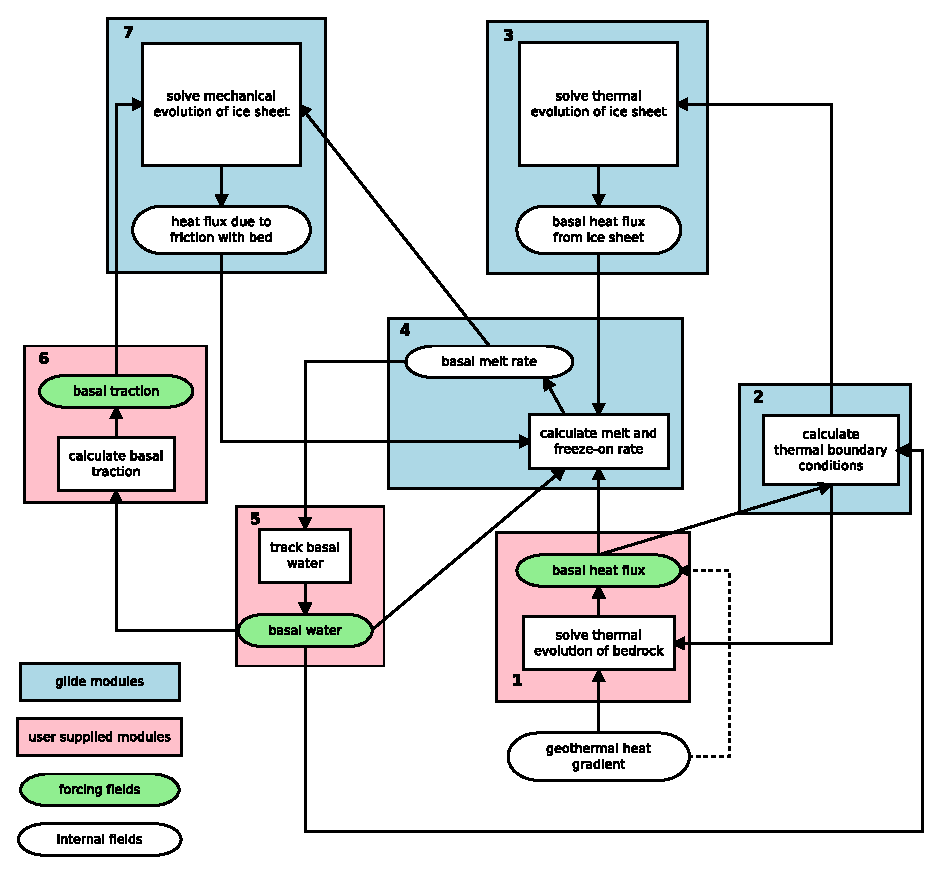
\includegraphics[width=\textwidth]{\dir/figs/basal_alg.eps}
  \caption{Flow diagram illustrating how the various modules communicate with each other by exchanging data fields.}
  \label{num.fig.bc_flow}
\end{figure}
The order of executions is then:
\begin{enumerate}
\item Find the basal heat flux by either solving the equation describing the thermal evolution of the lithosphere, \eqref{num.eq.diffu_rock}, or by using the geothermal heat flux directly. The upper boundary condition of \eqref{num.eq.diffu_rock} is the same as the lower boundary condition of the thermal evolution of the ice sheet.
\item Either (1) the lower boundary condition for the thermal evolution of the ice sheet is given by the basal heat flux from \emph{Step 1}; or (2) if melt water is present, the basal temperature is set to the pressure melting point of ice.
\item Calculate the temperature distribution within the ice sheet given the boundary condition found during \emph{Step 2} and the atmospheric BC.
\item Calculate a melt/freeze--on rate using Equation \eqref{bc.eq.meltrate} given the outgoing heat flux calculated during \emph{Step 3}, friction with the bed (calculated during the previous \emph{Step 7}) and the incoming heat flux from \emph{Step 1}. Freezing occurs only when there is basal water.
\item Track basal water. This is a user supplied module which can take any complexity. Inputs will typically be the melt/freeze--on rate determined during \emph{Step 4}.
\item Calculate the basal traction parameter. Again, this is a user supplied module which typically will involve the presence of basal water (calculated during \emph{Step 5}).
\item Solve the mechanical ice equations given basal traction parameter from \emph{Step 6}.
\end{enumerate}
Clearly, this scheme has the problem that heat is lost if the basal heat flux is such that more water could be frozen than is available. This might be avoided by iterating the process. On the other hand, the heat loss may be negligible if time steps are fairly small.

\section{Isostatic Adjustment}
The ice sheet model includes simple approximations for calculating isostatic adjustment. These approximations depend on how the lithosphere and the mantle are treated. For each subsystem there are two models. The lithosphere can be described as a
\begin{description}
\item[\textbf{local lithosphere:}] the flexural rigidity of the lithosphere is ignored, i.e. this is equivalent to ice floating directly on the asthenosphere;
\item[\textbf{elastic lithosphere:}] the flexural rigidity is taken into account;
\end{description}
while the mantle is treated as a
\begin{description}
\item [\textbf{fluid mantle:}] the mantle behaves like a non-viscous fluid, isostatic equilibrium is reached instantaneously;
\item [\textbf{relaxing mantle:}] the flow within the mantle is approximated by an exponentially decaying hydrostatic response function, i.e. the mantle is treated as a viscous half space.
\end{description}

\subsection{Calculation of ice-water load}
At each isostasy time-step, the load of ice and water is calculated, as an
equivalent mantle-depth ($L$). If the basal elevation is above sea-level, then the
load is simply due to the ice:
\begin{equation}
L=\frac{\rho_i}{\rho_m}H,
\label{load_land_ice}
\end{equation}
where $H$ is the ice thickness, with $\rho_i$ and $\rho_m$ being the densities
of the ice and mantle respectively. In the case where the bedrock is below
sea-level, the load is calculated is that due to a change in sea-level rise and/or
the presence of non-floating ice. When the ice is floating ($\rho_i
H<\rho_o(z_0-h)$), the load is only due to sea-level changes
\begin{equation}
L=\frac{\rho_o}{\rho_m}z_0,
\label{load_sea_float}
\end{equation}
whereas when the ice is grounded, it displaces the water, and adds an
additional load:
\begin{equation}
L=\frac{\rho_i H+\rho_o b_r}{\rho_m}.
\label{load_sea_grounded}
\end{equation}
here, $\rho_o$ is the density of sea water, $z_0$ is the change in sea-level
relative to a reference level and $b_r$ is the bedrock elevation relative to the
same reference level. The value of $b_r$ will be negative for submerged bedrock,
hence the plus sign in (\ref{load_sea_grounded}).

\subsection{Elastic lithosphere model}
This is model is selected by setting \texttt{lithosphere = 1} in the
configuration file. By simulatuing the deformation of the lithosphere, the
deformation seen by the aesthenosphere beneath is calculated. In the absence of this
model, the deformation is that due to Archimedes' Principle, as though the
load were floating on the aesthenosphere.

The elastic lithosphere model is based on work by \cite{Lambeck1980}, and its
implementation is fully described in \cite{Hagdorn2003}. The lithosphere
model only affects the geometry of the deformation --- the timescale for
isostatic adjustment is controlled by the aesthenosphere model. 

The load due to a single (rectangular) grid point is approximated as being
applied to a disc of the same area. The deformation due to a disc of ice of
radius $A$ and thickness $H$ is given by these expressions. For $r<A$:
\begin{equation} 
w(r)=\frac{\rho_i H}{\rho_m}\left[1+C_1\,\mathrm{Ber}\left(\frac{r}{L_r}\right)+C_2\,\mathrm{Bei}\left(\frac{r}{L_r}\right)\right],
\end{equation}
and for $r\geq A$:
\begin{equation}
w(r)=\frac{\rho_i
  H}{\rho_m}\left[D_1\,\mathrm{Ber}\left(\frac{r}{L_r}\right)+D_2\,\mathrm{Bei}\left(\frac{r}{L_r}\right)
+D_3\,\mathrm{Ker}\left(\frac{r}{L_r}\right)+D_4\,\mathrm{Kei}\left(\frac{r}{L_r}\right)\right],
\end{equation}
where $\mathrm{Ber}(x)$, $\mathrm{Bei}(x)$, $\mathrm{Ker}(x)$ and
$\mathrm{Kei}(x)$ are Kelvin functions of zero order, $L_r=(D/\rho_m
g))^{1/4}$ is the radius of relative stiffness, and $D$ is the flexural
rigidity. The constants $C_i$ and $D_i$ are given by
\begin{equation}
\begin{array}{rcl}
C_1&=&a\,\mathrm{Ker}'(a)\\
C_2&=&-a\,\mathrm{Ker}'(a)\\
D_1&=&0\\
D_2&=&0\\
D_3&=&a\,\mathrm{Ber}'(a)\\
D_4&=&-a\,\mathrm{Ber}'(a).
\end{array}
\end{equation}
Here, the prime indicates the first spatial derivative of the Kelvin functions.

\subsection{Relaxing aesthenosphere model}
If a fluid mantle is selected, it adjusts instantly to changes in lithospheric
loading. However, a relaxing mantle is also available.

%%% Local Variables: 
%%% mode: latex
%%% TeX-master: "isos"
%%% End: 



% ==========================
% MJH: An additional section not worth adding a new file for

\section{Time Step Ordering}

Relative to Glimmer-CISM 1.x, the order of operations on each time step has been
somewhat reorganized in CISM2.0.  This was done for consistency with the ordering
of operations used in Glissade and to eliminate discrepancies between time levels
applied in the model and the time levels written in output files.  
\textbf{These changes have only a minor impact on model results, but do result 
in output that will not be an exact match between the two model versions for the
same configuration and initial conditions.}

While unlikely to be of much interest to the average user, particularly if you are not
migrating from Glimmer-CISM 1.x, the details of these changes follow.
Specifically, in Glimmer-CISM 1.x, for a given time step, $H$ is advanced in time
relative to $T$ and $\vec{v}$, and, because a complete solve occurs even at the 
initial time, the output for the initial time is different than the input for 
the prognostic variables $H$ and $T$, even though no time step has occurred at 
that point.

In Glimmer-CISM 1.x, the time-stepping loop is organized as follows:
\begin{verbatim}
glide_initialise(): init T, H, v
do while (t < tend)
   glide_tstep_p1(): solve T
   glide_tstep_p2(): solve v, H
   glide_tstep_p3(): calculate some diagnostic variables, write output for time t
   advance time
end do
\end{verbatim}

\noindent This results in the following relation between the state of model variables and
the time level at which they are output:

%\begin{table}[h]
%\caption{Relation between state of model variables and output time level in Glimmer-CISM 1.x}
\begin{tabular}{lccc}
\hline
Output time:  & 0    & 1   & 2  \\
\hline
$T$  &  1                    &  2                    &  3  \\
$H$  &  1                    &  2                    &  3  \\
$v$  &  0                    &  1                    &  2  \\
\hline
\end{tabular}
%\end{table}
\\~\\  % hack to get a little more vertical separation here

In CISM 2.0, the time-stepping loop is now organized as follows:
\begin{verbatim}
initialize modules
initial diagnostic solve of v (and any other diagnostic variables like upper surface)
write output for time 0
do while (t <= tend)
   advance time
   solve column physics: T = f(H,T) 
   solve prognostic variables: advection of H=f(H,v), T=f(H,v)
   solve diagnostic variables: v=f(H,T)
   write output for time t
end do
\end{verbatim}

\noindent
This results in the following relation between the state of model variables and
the time level at which they are output:

%\begin{table}[h]
%\caption{Relation between state of model variables and output time level in CISM 2.0}
\begin{tabular}{lccc}
\hline
Output time:  & 0    & 1   & 2  \\
\hline
$T$  &  0                    &  1                    &  2  \\
$H$  &  0                    &  1                    &  2  \\
$v$  &  0                    &  1                    &  2  \\
\hline
\end{tabular}
%\end{table}


